\label{s:exp_retinogram_orientation_wrt_width}
% Compute orientation errors for lines of different widths
%
Because narrow vessels are interesting but occupy a small proportion of the vessel map, here we provide a breakdown of orientation errors for lines of different widths. To estimate the vessel widths, we computed the distance transform of the known vessel mask and set the width at every vessel pixels to that of the nearest centreline pixel.

\begin{figure}[t]
\centering
\def\figwidth{0.75\columnwidth}
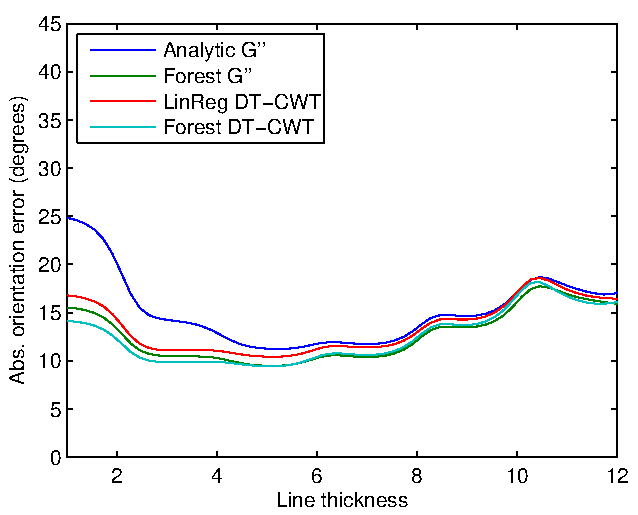
\includegraphics[width=\figwidth]{\figpath/retina/thickness_vs_error-summ} 
%
\caption{Orientation estimation results for selected methods over pixels along the centre of the vessel: Kernel estimate of mean error with respect to line thickness.}
\label{f:retinogram_orientation_wrt_width}
\end{figure}

We visualize this relationship using a one dimensional kernel smoother (\fref{f:retinogram_orientation_wrt_width}) and see that errors are similar for the thicker vessels (where there is more image information with which to estimate orientation and thus we expect all methods to perform well) but that the regression reduces error considerably for the narrower vessels. Interpreting results for vessels with a width of more than approximately 12 pixels is difficult because they are rare, which leads to high variability in the kernel estimate of error, and because the vessel width exceeds the central region of our largest filter. These vessels, however, are typically of less interest to the retinopathy community.
